\documentclass[border=2pt]{standalone}
\usepackage[dvipsnames,svgnames,x11names]{xcolor}
\usepackage{tikz}
\usetikzlibrary{petri,positioning,arrows.meta}
\begin{document}
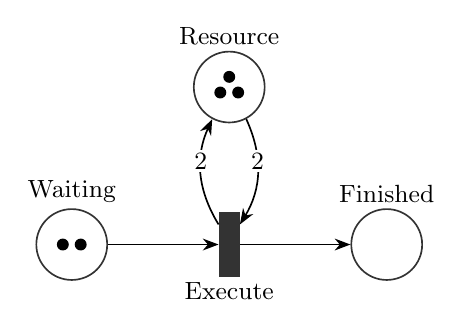
\begin{tikzpicture}[x=1cm,y=1cm,>=Stealth,font=\small]
\node[place,minimum size=9mm,line width=0.6pt,draw=black!80,fill=white,tokens=2] (waiting) at (0,0) {};
\node[above=2pt of waiting,inner sep=0pt] {Waiting};
\node[place,minimum size=9mm,line width=0.6pt,draw=black!80,fill=white,tokens=3] (resource) at (2,2) {};
\node[above=2pt of resource,inner sep=0pt] {Resource};
\node[place,minimum size=9mm,line width=0.6pt,draw=black!80,fill=white,tokens=0] (finished) at (4,0) {};
\node[above=2pt of finished,inner sep=0pt] {Finished};
\node[transition,minimum width=2.5mm,minimum height=8mm,line width=0.6pt,draw=black!80,fill=black!80] (execute) at (2,0) {};
\node[below=2pt of execute,inner sep=0pt] {Execute};
\draw[->,line width=0.6pt] (waiting) -- (execute);
\draw[->,line width=0.6pt] (resource) to[bend left=28] node[midway,above,fill=white,inner sep=1pt] {2} (execute);
\draw[->,line width=0.6pt] (execute) to[bend left=28] node[midway,above,fill=white,inner sep=1pt] {2} (resource);
\draw[->,line width=0.6pt] (execute) -- (finished);
\end{tikzpicture}
\end{document}
